\chapter{Datapath Multiciclo}

\section{Schema}
\begin{center}
    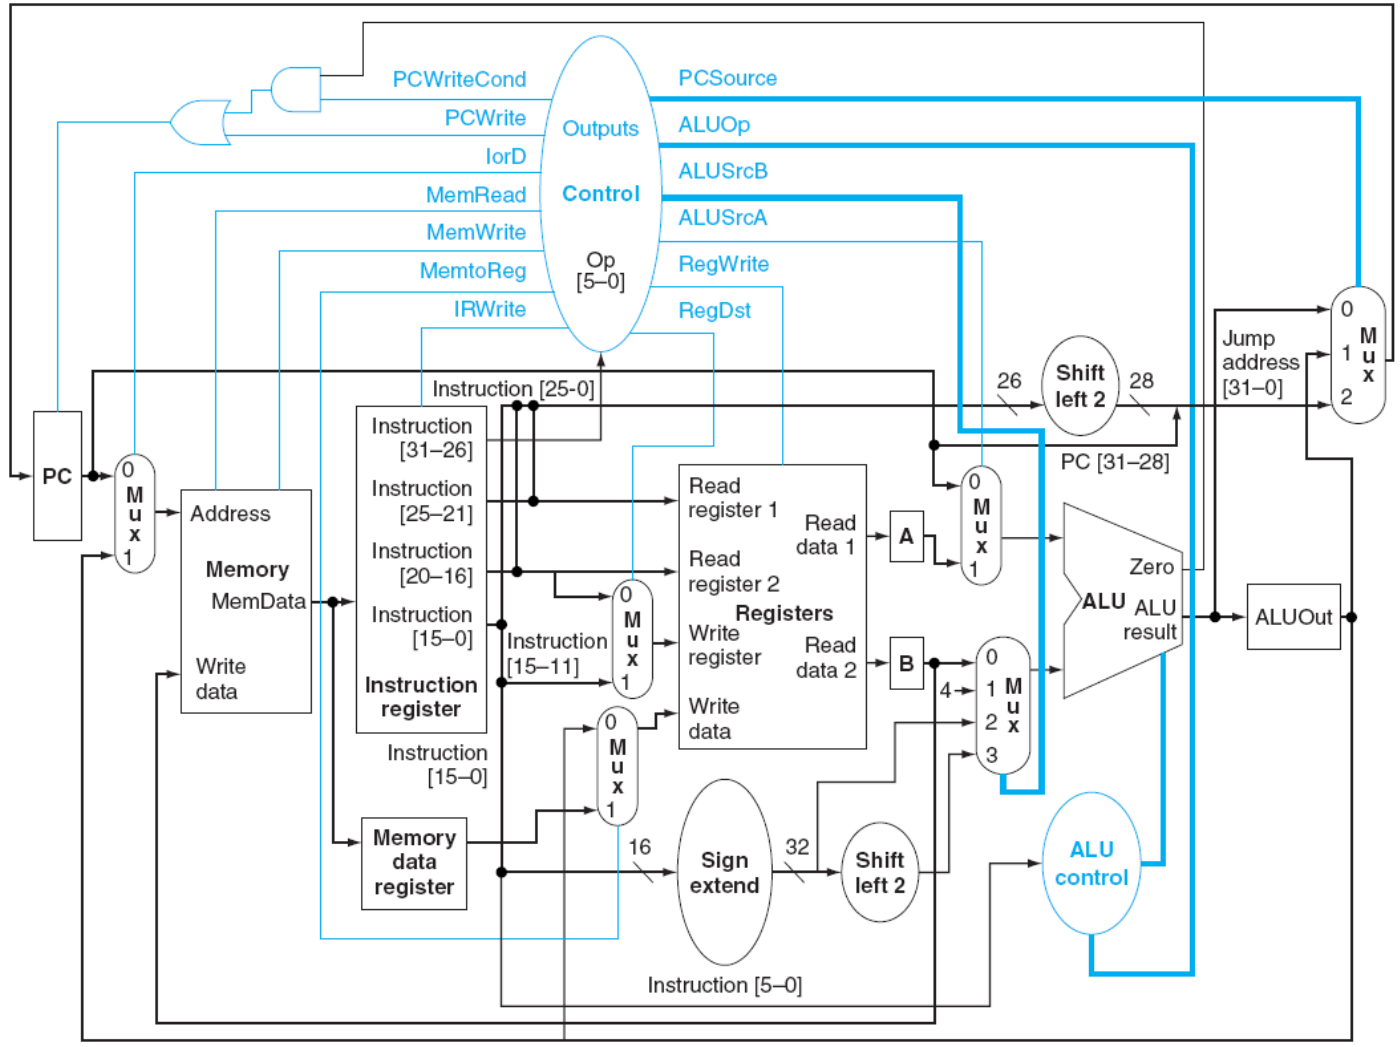
\includegraphics[scale=0.375]{Immagini/Datapath Multiciclo.png}
\end{center}

\newpage

\section{Componenti}
\subsection{Unità Funzionali}
\begin{itemize}
    \item \textbf{Memoria}: \\
        Un' unità unificata che contiene sia istruzioni che dati.\\
        Sulla base dell'indirizzo ricevuto in input, restituisce in output l'istruzione o il dato letto, oppure memorizza il dato (WriteData) nel caso di un'istruzione

    \item \textbf{Register File}: \\
        Un banco composto da 32 registri che contengono i dati utilizzati durante l'esecuzione delle istruzioni.\\
        Restituisce in output il contenuto dei due registri letti e, nel caso di istruzioni \texttt{load} o \texttt{R-Type}, scrive il dato ricevuto in input nel registro specificato

    \item \textbf{ALU}: \\
        Si occupa di eseguire le operazioni aritmetico-logiche richieste, come il calcolo del valore di branch o l'incremento del PC

    \item \textbf{Sign extend}: \\
        Unità per l'estensione del segno a 32 bit

    \item \textbf{Shift left 2}: \\
        Unità per scorrere i bit a sinistra di 2 posizioni
\end{itemize}

\subsection{Registri}
\begin{itemize}
    \item \textbf{PC - Program Counter}: \\
        Mantiene l'indirizzo dell'istruzione da eseguire

    \item \textbf{IR - Instruction Register}: \\
        Memorizza i bit dell'istruzione letta dalla memoria

    \item \textbf{Memory data register}: \\
        Memorizza il dato letto dalla memoria, utilizzato ad esempio per le istruzioni di tipo \texttt{load}

    \item \textbf{Registro A e Registro B}: \\
        Registri temporanei in cui vengono scritti i valori provenienti dal register file durante la fase di fetch (il valore del registro sorgente \texttt{\$ra} in A, il valore \texttt{\$rt} in B)

    \item \textbf{ALUOut}: \\
        Memorizza temporaneamente l'output generato dalla ALU
\end{itemize}

\subsection{Multiplexer}
Sono necessari per selezionare dinamicamente i percorsi dei dati nei diversi cicli di esecuzione

\begin{itemize}
    \item \textbf{MUX A}: \\
        Seleziona l'indirizzo di memoria a cui accedere tra il PC (per leggere un'istruzione) e l'output della ALU (per le istruzioni \texttt{load} o \texttt{store})

    \item \textbf{MUX B}: \\
        Seleziona il gruppo di bit dell'IR che indica il registro in cui scrivere (IR per le \texttt{load}, IR per le \texttt{R-Type})

    \item \textbf{MUX C}: \\
        Seleziona la sorgente del dato da scrivere nel register file (MemoryDataRegister per le \texttt{load}, ALUOut per le \texttt{R-Type})

    \item \textbf{MUX D}: \\
        Seleziona il primo operando dell'operazione aritmetico-logica della ALU tra il PC e il registro A

    \item \textbf{MUX E}: \\
        Seleziona il secondo operando della ALU tra il registro B, il valore costante 4, l'estensione in segno dell'IR[15:0], oppure l'estensione in sogno "2-shifted"

    \item \textbf{MUX F}: \\
        Seleziona il valore per l'aggionamento del PC tra l'output della ALU (PC + 4), il contenuto di ALUOut, o il jump target address
\end{itemize}

\section{Segnali di controllo}

\subsection{Segnali di Abilitazione (a 1 bit)}
Questi segnali controllano la scrittura o la lettura negli elementi di stato (memoria e registri). Un valore alto (1) attiva l'azione, un valore basso (0) la disabilita.

\begin{itemize}
    \item \textbf{MemRead}: Abilita la lettura dalla memoria principale.
    \begin{itemize}
        \item \textbf{1}: Legge l'istruzione o il dato dall'indirizzo specificato (utilizzato nello stato di \textit{fetch} per leggere l'istruzione o nell'istruzione \texttt{load}).
    \end{itemize}
    \item \textbf{MemWrite}: Abilita la scrittura nella memoria principale.
    \begin{itemize}
        \item \textbf{1}: Scrive il valore presente nell'ingresso "Write data" all'indirizzo specificato (utilizzato nell'istruzione \texttt{store}).
    \end{itemize}
    \item \textbf{IRWrite}: Abilita la scrittura nell'Instruction Register (IR).
    \begin{itemize}
        \item \textbf{1}: Memorizza l'istruzione appena letta dalla memoria (utilizzato solo nella fase di \textit{fetch}).
    \end{itemize}
    \item \textbf{RegWrite}: Abilita la scrittura nel Register File.
    \begin{itemize}
        \item \textbf{1}: Il dato presente in "Write data" viene scritto nel registro di destinazione selezionato (utilizzato alla fine delle istruzioni R-type, \texttt{load} o \texttt{swap}).
    \end{itemize}
    \item \textbf{PCWrite}: Abilita l'aggiornamento incondizionato del Program Counter (PC).
    \begin{itemize}
        \item \textbf{1}: Il PC memorizza un nuovo valore (utilizzato nel \textit{fetch} per salvare PC+4 o nei salti incondizionati come \texttt{jump}).
    \end{itemize}
    \item \textbf{PCWriteCond}: Abilita l'aggiornamento condizionato del Program Counter.
    \begin{itemize}
        \item \textbf{1}: Il PC viene aggiornato solo se la ALU restituisce il segnale \texttt{Zero = 1} (utilizzato per i salti condizionati come \texttt{beq}).
    \end{itemize}
\end{itemize}

\subsection{Segnali di Selezione Multiplexer a 2 vie (a 1 bit)}
Questi segnali fungono da selettori per i Multiplexer (MUX) che hanno due soli ingressi.

\begin{itemize}
    \item \textbf{IorD (MUX A)}: Seleziona la sorgente dell'indirizzo da inviare alla memoria.
    \begin{itemize}
        \item \textbf{0}: Seleziona il PC (utilizzato per leggere un'istruzione nella fase di \textit{fetch}).
        \item \textbf{1}: Seleziona l'output della ALU (utilizzato per l'esecuzione di istruzioni \texttt{load} o \texttt{store}).
    \end{itemize}
    \item \textbf{RegDst (MUX B)}: Seleziona quale parte dell'istruzione indica il registro in cui scrivere.
    \begin{itemize}
        \item \textbf{0}: Seleziona IR[20:16] (utilizzato per le istruzioni \texttt{load}).
        \item \textbf{1}: Seleziona IR[15:11] (utilizzato per le istruzioni R-type).
    \end{itemize}
    \item \textbf{ALUSrcA (MUX D)}: Seleziona il primo operando per la ALU.
    \begin{itemize}
        \item \textbf{0}: Seleziona il PC (utilizzato per l'incremento di +4 o per calcolare il valore di branch).
        \item \textbf{1}: Seleziona il registro A (utilizzato per istruzioni R-type, branch o \texttt{jump} con registro).
    \end{itemize}
    \item \textbf{MemtoReg (MUX C)}: Seleziona la sorgente del dato da scrivere nel register file.
    \begin{itemize}
        \item \textbf{0}: Seleziona ALUOut (utilizzato per le istruzioni R-type).
        \item \textbf{1}: Seleziona MemoryDataRegister (utilizzato per le istruzioni \texttt{load}).
        \item \textit{Nota}: In varianti dello schema (es. per l'istruzione \texttt{swap}), questo segnale può essere esteso a 2 bit per selezionare direttamente i registri A o B.
    \end{itemize}
\end{itemize}

\subsection{Segnali di Controllo a 2 bit (Multiplexer complessi e ALU)}
Questi segnali controllano Multiplexer a 3 o 4 vie, oppure l'unità di controllo della ALU.

\begin{itemize}
    \item \textbf{ALUSrcB (MUX E)}: Seleziona il secondo operando per la ALU.
    \begin{itemize}
        \item \textbf{00}: Seleziona il registro B (utilizzato per istruzioni R-type e branch).
        \item \textbf{01}: Seleziona la costante 4 (utilizzato per l'aggiornamento del PC nella fase di \textit{fetch}).
        \item \textbf{10}: Seleziona l'estensione del segno di IR[15:0] a 32 bit (utilizzato per istruzioni di accesso a memoria \texttt{lw}/\texttt{sw} o calcoli immediati).
        \item \textbf{11}: Seleziona l'estensione del segno di IR[15:0] shiftato a sinistra di 2 posizioni (utilizzato per pre-calcolare il valore di branch).
    \end{itemize}
    \item \textbf{PCSource (MUX F)}: Seleziona il valore con cui aggiornare il PC.
    \begin{itemize}
        \item \textbf{00}: Seleziona l'output diretto della ALU, ovvero PC+4.
        \item \textbf{01}: Seleziona il contenuto di ALUOut, ovvero l'indirizzo di branch calcolato (PC + 2 shifted sign-extended branch field).
        \item \textbf{10}: Seleziona il jump target address (indirizzo shiftato concatenato al PC).
    \end{itemize}
    \item \textbf{ALUOp}: Segnale inviato all'unità \texttt{ALU control} per decidere l'operazione aritmetico-logica da eseguire.
    \begin{itemize}
        \item \textbf{00}: Forza l'esecuzione di un'addizione (utilizzato nel \textit{fetch} per PC+4, nel \textit{decode}, e per il calcolo indirizzi memoria).
        \item \textbf{01}: Forza l'esecuzione di una sottrazione (utilizzato nello stato di esecuzione per verificare l'uguaglianza nel branch).
        \item \textbf{10}: Delega la decisione al campo \texttt{funct} (IR[5:0]) dell'istruzione (utilizzato per le istruzioni R-type).
    \end{itemize}
\end{itemize}

\subsection{Segnali per la Gestione delle Eccezioni (Co-processore 0)}
Quando il datapath viene esteso per gestire le eccezioni sincrone e asincrone, vengono aggiunti ulteriori segnali specifici controllati dalla FSM.

\begin{itemize}
    \item \textbf{EPCWrite}: Se a 1, abilita la scrittura dell'indirizzo dell'istruzione che ha causato l'eccezione nel registro \texttt{EPC}.
    \item \textbf{CauseWrite}: Se a 1, abilita la scrittura del tipo di eccezione nel registro \texttt{Cause}.
    \item \textbf{IntCause}: Identifica la causa specifica dell'eccezione (es. 0 per istruzione non valida, 1 per overflow aritmetico) per codificarla all'interno del registro \texttt{Cause}.
\end{itemize}

\section{Metodologia di clocking}
\begin{itemize}
    \item Ciclo di lunghezza fissa
    \item Ogni istruzione viene eseguita in più cicli di clock
    \item Istruzioni di tipo diverso vengono eseguito in un numero di cicli di clock diverso
    \item Le unità funzionali vengono usate più volte durante l'esecuzione della stessa istruzione in cicli di clock differenti
    \item Si usano registri aggiuntivi per memorizzare i risultati parziali nell'esecuzione delle istruzioni
\end{itemize}

\section{Passaggi per l'esecuzione di una istruzione}
\begin{enumerate}
    \item \textbf{Fetch}:
        \begin{enumerate}[label=\theenumi.\arabic*]
            \item Legge l'istruzione dalla memoria e la salva in un registro dedicato (IR - Instruction Register)
            \item L'indirizzo di memoria che indica l'istruzione da leggere si trova nel registro Program Counter (PC)
            \item Dopo la lettura dell'istruzione in PC viene incrementato di 4 (usando l'ALU) per indicare la prossima istruzione da leggere
        \end{enumerate}

    \item \textbf{Decode}:
        \begin{enumerate}[label=\theenumi.\arabic*]
            \item Decodificare i vari campi dell'istruzione per decidere quali sono i passi necessari per la sua esecuzione
        \end{enumerate}

    \item \textbf{Execute}:
        \begin{enumerate}[label=\theenumi.\arabic*]
            \item Esegue i passi necessari per eseguire l'istruzione
        \end{enumerate}
\end{enumerate}

Le operazioni di Fetch e Decode sono \textbf{uguali per tutti i tipi d'istruzione}, mentre l'operazione Execute dell'operazione di Execute cambia in base al tipo di istruzione da eseguire

\newpage

\section{FSM}
\begin{minipage}{0.45\textwidth}
    \subsection{Circuito sequenziale per il controllo}
    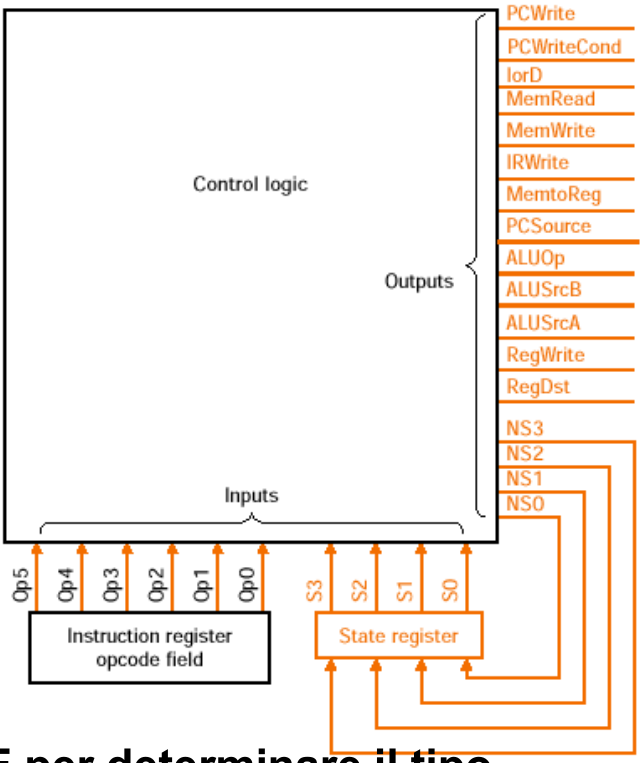
\includegraphics[scale=0.4]{Immagini/Schema FSM.png}
\end{minipage}
\hfil
\begin{minipage}{0.45\textwidth}
    \subsection{FSM}
    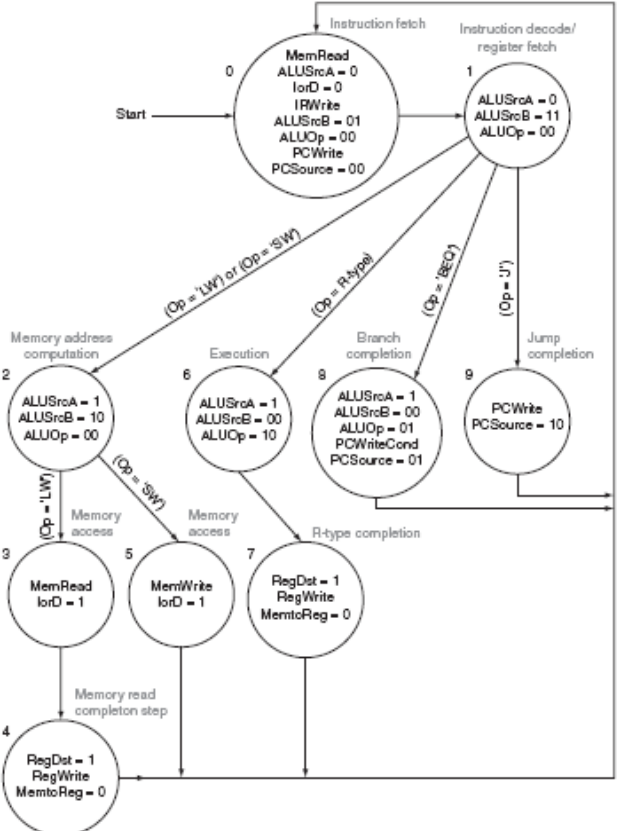
\includegraphics[scale=0.4]{Immagini/DFA SFM.png}
\end{minipage}

\subsection{Spiegazione}
\begin{itemize}
    \item Controllo a due livelli:
        \begin{itemize}
            \item Si usa \textbf{OPCODE} per determinare il tipo dell'istruzione
            \item Per le \uline{istruzioni R-Type} si usa anche il \textbf{funct}
        \end{itemize}
    
    \item State register memorizza lo stato corrente
    
    \item Blocco combinatorio (PLA) per il calcolo di NEXT\_STATE e OUTPUT
\end{itemize}

\newpage

\section{Fetch}
\subsection{Spiegazione}
Durante questo ciclo, il processore esegue contemporaneamente 2 compiti principali:
    \begin{itemize}
        \item Preleva l'istruzione dalla memoria
        \item Prepara il Program Counter (PC) per l'istruzione successiva
    \end{itemize}

L'intera operazione \uline{viene svolta in un singolo ciclo di clock}
\subsection{Componenti utilizzati}
\begin{itemize}
    \item Memoria
    \item Instruction Register
    \item Program Counter
    \item ALU
\end{itemize}


\subsection{Procedura}
\begin{enumerate}
    \item \textbf{Ciclo di clock 1}
        \begin{enumerate}[label=\theenumi.\arabic*]
            \item Usando l'indirizzo salvato all'interno del Program Counter prelevo l'istruzione da eseguire dalla memoria e la salvo all'interno dell'Instruction Register
            \item Utilizzando l'ALU aggiorno il PC a PC+4
        \end{enumerate}
\end{enumerate}

\subsection{Segnali}
\begin{itemize}
    \item \textbf{MemRead} per leggere dalla memoria
    \item \textbf{IRWrite} per scrivere nell'Instruction Register
    \item \textbf{IorD} per indicare da dove leggere dalla memoria
    \item \textbf{ALUSrcA, ALUSrcB, ALUop} per incrementare il PC
    \item \textbf{PCSource, PCWrite} per salvare il nuovo valore del PC al suo interno
\end{itemize}

\newpage

\section{Decode}
\subsection{Spiegazione}
Durante questo ciclo, il processore esegue contemporaneamente 2 compiti principali:
\begin{itemize}
    \item Il processore MIPS legge i vari campi dell'istruzione
    \item Il processore identifica il tipo di istruzione da eseguire usando l'opcode ed eventualmente anche il funct
\end{itemize}

L'intera operazione \uline{viene svolta in un singolo ciclo di clock}

\subsection{Componenti utilizzati}
\begin{itemize}
    \item Instruction Register
    \item Registro A
    \item Registro B
    \item ALUOut
    \item Sign Extend
\end{itemize}


\subsection{Procedura}
\begin{enumerate}
    \item[2.] \textbf{Ciclo di clock 2}
        \begin{enumerate}[label=\theenumi.\arabic*]
            \item [2.1] Il registro A usa i bit dal 25 al 21 dell'Instruction Register come eventuale dato per un istruzione futura
            \item [2.2] Il registro B usa i bit dal 20 al 16 dell'Instruction Register come eventuale dato per un istruzione futura
            \item [2.3] L'instruction register inserisci i bit dal 15 al 0 all'interno del sign extend e shift left 2, questo valore viene poi salvato all'interno di ALUOut per un eventuale calcolo di indirizzo di salto.
            \item [2.4] L'instruction register inserisce i bit dal 31 al 26 all'internodel FSM per decidere l'istruzione da effetuare utilizzando l'opcode
        \end{enumerate}
\end{enumerate}

\subsection{Segnali}
\begin{itemize}
    \item \textbf{ALUSrcA, ALUSrcB, ALUOp} per il calcolo di un eventuale indirizzo di branch
\end{itemize}

\newpage

\section{Execute per le istruzioni jump}
\subsection{Spiegazione}
Durante questa istruzione il processore esegue un solo compito:
\begin{itemize}
    \item Cambia l'indirizzo della prossima istruzione da eseguire con quella dell'indirizzo di salto calcolato durante la decode
\end{itemize}

L'intera istruzione \uline{viene completata in un singolo ciclo di clock}

\subsection{Componenti utilizzati}
\begin{itemize}
    \item Program Counter
    \item Instruction Register
\end{itemize}

\subsection{Procedura}
\begin{enumerate}
    \item[3.] \textbf{Ciclo di clock 3}
        \begin{enumerate}[label=\theenumi.\arabic*]
            \item [3.1] Il PC viene sovrascritto con l'indirizzo calcolato dall'ALU utilizzando i bit dal 31 al 28 del PC sommati ai bit dal 25 allo 0 dell'Instruction Register
        \end{enumerate}
\end{enumerate}

\subsection{Segnali}
\textbf{PCWrite, PCSource} per scrivere all'interno del PC

\newpage

\section{Execute beq}
\subsection{Spiegazione}
Durante questa istruzione il processore esegue 2 compiti:
\begin{itemize}
    \item Effettua il confronto tra i 2 valori 
    \item Eventualmente in base all'esito del confronto aggiorna il Program Counter
\end{itemize}

L'esecuzione di questa istruzione \uline{viene completata in un solo ciclo di clok}

\subsection{Componenti utilizzati}
\begin{itemize}
    \item Registro A
    \item Registro B
    \item ALUOut
\end{itemize}

\subsection{Procedura}
\begin{enumerate}
    \item[3.] \textbf{Ciclo di clock 3}
        \begin{enumerate}[label=\theenumi.\arabic*]
            \item [3.1] Il PC viene sovrascritto con l'indirizzo calcolato dall'ALU utilizzando i bit dal 31 al 
        \end{enumerate}
\end{enumerate}

\subsection{Segnali}
\begin{itemize}
    \item \textbf{ALUSrcA, ALUSrcB, ALUOp} per la comparazione tra A e B
    \item \textbf{PCWriteCond, PCSource} per scrivere all'interno del PC
\end{itemize}

\newpage

\section{Execute R-Type}
\subsection{Spiegazione}
Durante questa istruzione il processore esegue 2 compiti:

\begin{itemize}
    \item Effettuare l'operazione aritmetico logica definita dall'istruzione
    \item Salvare il risultato dell'operazione effettuata
\end{itemize}

L'esecuzione di questo tipo d'istruzioni \uline{dura 2 cicli di clock}

\subsection{Componenti utilizzati}
\begin{itemize}
    \item Registro A
    \item Registro B
    \item ALUOut
    \item Instruction Register
    \item Registro di destinazione dell'operazione
\end{itemize}

\subsection{Procedura}
\begin{enumerate}
    \item[3.] \textbf{Ciclo di clock 3}
        \begin{enumerate}[label=\theenumi.\arabic*]
            \item [3.1] Viene effettuata l'istruzione 
            \item [3.2] Il risultato dell'istruzione appena avvenuta viene salvato all'interno di ALUOut
        \end{enumerate}
    \item [4.] \textbf{Ciclo di clock 4}
        \begin{enumerate}
            \item [4.1] I contenuti di ALUOut vengono salvati nel registro di destinazione all'interno del Register file. L'indirizzo di questo registro di destinazione è specificato dai bit dal 15 all'11 dell'Instruction Register
        \end{enumerate}
\end{enumerate}

\subsection{Segnali}
\begin{itemize}
    \item \textbf{ALUScrA, ALUSrcB, ALUOp} per effettuare il calcolo aritmetico logico
    \item \textbf{RegWrite} per poter scrivere nel Register File
    \item \textbf{RegDest} per indicare il registro da scrivere
    \item \textbf{MemToReg} per scrivere il valore nel ALUOut
\end{itemize}

\newpage

\section{Execute Store Word}

\subsection{Spiegazione}
Durante questa istruzione il processore esegue 2 compiti:
\begin{itemize}
    \item Calcolare l'indirizzo dove salvare il dato
    \item Scrivere il dato in memoria
\end{itemize}

L'esecuzione di questa istruzione dura \uline{2 cicli di clock}

\subsection{Componenti utilizzati}
\begin{itemize}
    \item Registro A
    \item \textbf{Eventualmente} Registro B
    \item Sing extend
    \item Instruction Register
    \item ALUOut
    \item Memory data register \textbf{oppure} Memory
\end{itemize}

\subsection{Procedura}
\begin{enumerate}
    \item[3.] \textbf{Ciclo di clock 3}
        \begin{enumerate}[label=\theenumi.\arabic*]
            \item [3.1] Utilizzo il registro A e i bit dal 15 allo 0 dell'Instruction Register per calcolare l'indirizzo a in cui salvare il dato
            \item [3.2] Salvo l'indirizzo calcolato all'interno di ALUOut
        \end{enumerate}
    \item [4.] \textbf{Ciclo di clock 4}
        \begin{enumerate} [label=\theenumi.\arabic*]
            \item [4.1] In questo ciclo avviene l'effettiva scrittura del dato in memoria.\\ Per fare ciò, il multiplexer A seleziona l'output della ALU come indirizzo di memoria a cui accedere.\\ Il processore provvederà quindi a salvare in tale indirizzo il dato desiderato
        \end{enumerate}
\end{enumerate}

\subsection{Segnali di controllo}
\begin{itemize}
    \item \textbf{ALUSrcA, ALUSrcB, ALUOp} per il calcolo dell'indirizzo di memoria
    \item \textbf{IorD} per indicare l'indirizzo di memoria
    \item \textbf{MemWrite} per scrivere nella memoria
\end{itemize}

\newpage

\section{Execute Load Word}
\subsection{Spiegazione}
Durante questa istruzione il processore esegue 3 compiti:
\begin{itemize}
    \item Calcolare l'indirizzo dov'è contenuto il dato da leggere
    \item Legge il dato dalla memoria
    \item Riscrivere il dato appena letto all'interno del Register File
\end{itemize}

\subsection{Componenti utilizzati}
\begin{itemize}
    \item Registro A
    \item Registro B
    \item Sign extend
    \item Instruction Register
    \item ALUOut
    \item Memory Data Register
\end{itemize}

\subsection{Procedura}
\begin{enumerate}
    \item[3.] \textbf{Ciclo di clock 3}
        \begin{enumerate}[label=\theenumi.\arabic*]
            \item [3.1] Utilizzo il registro A e i bit dal 15 allo 0 dell'Instruction Register per calcolare l'indirizzo da cui leggere il dato
            \item [3.2] Salvo l'indirizzo calcolato all'interno di ALUOut
        \end{enumerate}
    \item [4.] \textbf{Ciclo di clock 4}
        \begin{enumerate} [label=\theenumi.\arabic*]
            \item [4.1] All'interno del Memory Data Register viene salvato il contenuto della cella di memoria con l'indirizzo salvato all'interno del registro ALUOut
        \end{enumerate}
    \item [5.] \textbf{Ciclo di clock 5}
        \begin{enumerate} [label=\theenumi.\arabic*]
            \item [5.1] In questo ultimo ciclo viene fatto il write back, riscrivendo all'interno del Instrucion Register nei bit dal 20 al 16 l'indirizzo in cui riscrivere i contenuti conservati all'interno del Memory Data Register
        \end{enumerate}
\end{enumerate}

\subsection{Segnali}
\begin{itemize}
    \item \textbf{ALUSrcA, ALUSrcB, ALUOp} per il calcolo dell'indirizzo di memoria
    \item \textbf{IorD} per indicare l'indirizzo di memoria
    \item \textbf{MemRead} per leggere dalla memoria
    \item \textbf{RegWrite} per poter scrivere nel Register File
    \item \textbf{RegDest} per indicare in registro da scrivere
    \item \textbf{MemToReg} per scrivere il valore dalla memoria
\end{itemize}